\section{Aufgabe 1: Entscheidungsbäume}
\subsection{Feature Engineering}

\subsection{Analyse der Zielvariable}
%TODO: Vll nicht der beste Einstieg?}
Wie Abbildung \ref{fig:disc_target_variable} entnommen werden kann ist Ausprägung der Zielvariable ungleich auf beide Klassen verteilt. Die Klassifizierungsgenauigkeit eines Modells muss demnach unter Berücksichtigung der sogenannten \emph{Null Accuracy} bewertet werden. Unter \emph{Null Accuracy} versteht man die Genauigkeit eines Modells, dass unabhängig von allen Eingaben immer die am häufigsten auftretende Klasse vorhersagt. In unserem Fall würde ein Modell, welches immer Regen vorhersagt, eine Klassifizierungsgenauigkeit von 79,39\% erreichen.

\begin{figure}[h]
	\centering
	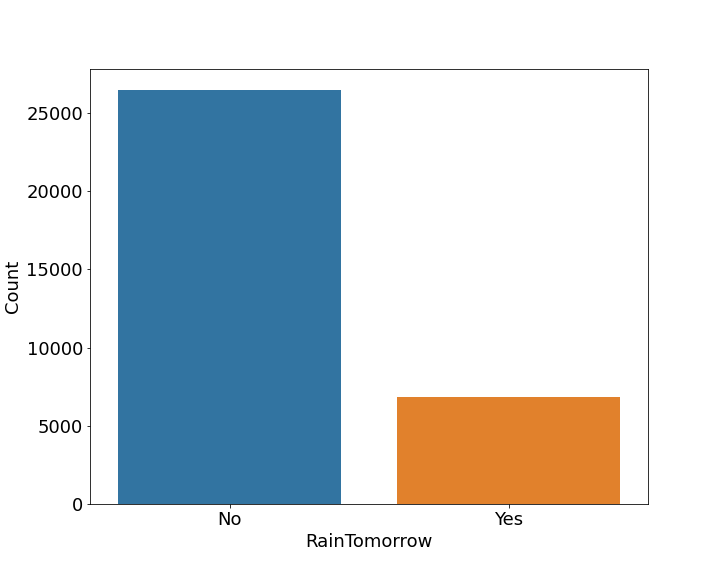
\includegraphics[width = 0.5\textwidth]{Bilder/distribution_target_variable}
	\caption{Entschidungsbaum mit Default-Einstellungen}
	\label{fig:disc_target_variable}
\end{figure}

\subsubsection{Fehlende Werte}
%TODO: Gesamter Absatz noch super holprig
Zunächst wurde der betrachtete Datensatz von fehlenden Werten bereinigt. Im ersten Schritt werden 834 Beobachtungen, welche keinen Wert für die Zielvariable \emph{RainTomorrow} aufweisen, aus dem Datensatz entfernt. Damit wurde die Anzahl an Beobachtungen auf 33402 reduziert.\\
\noindent \hspace*{7mm}
In einem nächsten Schritt werden die Spalten aus dem Datensatz entfernt, in denen mehr als 40\% der beinhaltenden Variablen keine validen Werte aufweisen. Namentlich werden somit die Spalten \emph{Evaporation, Sunshine, Cloud9am} sowie \emph{Cloud3pm} aus dem Datensatz entfernt. Der Schwellwert von 40\% wurde empirisch festgelegt und hat zu den besten Klassifizierungsergebnissen geführt.\\
\noindent \hspace*{7mm}
Des Weiteren werden Beobachtungen aus dem Datensatz entfernt, von denen mehr als 50\% der Variablen keine validen Werte zeigen. Das betrifft 55 Beobachtungen, sodass die Gesamtanzahl an Beobachtungen 33347 beträgt. Durch die ersten beiden Schritte wurden lediglich ca. 3\% der Beobachtungen entfernt.\\
\noindent \hspace*{7mm}
Die übrig gebliebenen Datensätze sind noch immer nicht frei von fehlenden Werten. Um diese zu ersetzen werden für kategorische und numerische Variablen verschiedene Strategien verfolgt. Für die \emph{Imputation} numerischer Werten wird der Median der jeweiligen Variablen verwendet, da dieser im Vergleich zum Mittelwert robuster gegenüber Ausreißern ist. Für kategorielle Variablen hingegen wird der am häufigsten vorkommende Wert verwendet. Wichtig bei der Ermittlung des Medians bzw. des häufigsten Wertes ist, dass dieser ausschließlich getrennt für Trainigs- und Testdaten ermittelt wird. Die Ermittlung auf Basis des gesamten Datensatzes würde eine \emph{Test-Train-Leakage} darstellen und ist zu vermeiden. Es muss davon ausgegangen werden, dass die Testdaten nicht bekannt sind. Die jeweils ermittelten Werte werden dann auf die Trainings- und Testdaten angewendet.

\subsubsection{Merkmalsaufteilung}
Das Feld \emph{Datum} wurde in die Merkmale \emph{Year, Month} und \emph{Day} aufgeteilt.

\subsubsection{Merkmalserstellung}
Eine weit verbreitete Technik des Feature Engineerings ist die Erstellung zusätzlicher Merkmalen. Somit wurde die Variable \emph{MinMaxDiff} erstellt, welche die Differenz zwischen der minimalen und der maximalen Tages-Temperatur angibt. In gleicher Weise wurden die Variablen \emph{PressureDiff, HumidityDiff und WindSpeedDiff} erstellt.

\subsubsection{Diskretisierung}
Die Diskretisierung eines Merkmals kann eine Überanpassung bei der Erstellung von Modellen verhindern, indem der Wertebereich des Merkmals minimiert und somit generalisiert wird. Es sollte beachtet werden, dass der Informationsverlust durch die Diskretisierung nicht zu hoch ausfällt.\\
\noindent \hspace*{7mm}
Zu Testzwecken wird das neu erstellte Merkmal \emph{Month} in zwei weiteren Merkmalen diskretisiert. Zum einen wird das kategorische Merkmal \emph{Season} erstellt, welches angibt,  in welcher Jahreszeit der Monat liegt. Zum anderen gibt das Boolean Merkmal \emph{RainyMonth} an, ob es sich um einen in Erwartung regenreichen Monat handelt.

\subsubsection{Kodierung kategorischer Werte}
Um kategorische Werte für weitere Analysen verwenden zu können, müssen diese in numerische Werte umkodiert werden. Hierbei wurden die folgenden Strategien Angewendet:
\begin{description}
	\item[Binäre Kodierung]\hfill \\
	%TODO: Das hört sich hoprig an.
	Die Zielvariable \emph{RainTomorrow}, sowie die Variable \emph{RainToday} liegen mit den binären Ausprägungen \emph{Yes} und \emph{No} vor. Die binären Werte wurden in eine numerische Darstellung umgewandelt
	\item[One-Hot-Kodierung]\hfill \\ 
	%TODO: auch sholprig
	Das neu diskretisierte Merkmal \emph{Season} wird mittels \emph{One-Hot Encoding} in drei Boolean Spalten aufgeteilt. Eine einfache Zuteilung eines Zahlenwertes pro auftretender Variablenausprägung hat den Nachteil, dass dadurch eine metrische numerische Variable für ein gegebenenfalls nicht metrisch interpretierbares Merkmal entsteht. Für Entscheidungsbäume wäre dies kein Problem, jedoch sollte das Feature Engineering weitgehend unabhängig von dem verwendeten Klassifizierungsalgorithmus durchgeführt werden.
	\item[Ziel-Kodierung]\hfill \\ 
	%TODO: Deutsch oder Englisch? Bedingte Wsl. vll als Mathematische schreibweise? 
	Mit Hilfe des \emph{Target Encodings} werden die Merkmale \emph{Location, WindGustDir, WindDir9am} und \emph{WindDir3pm} verarbeitet. Dabei werden den jeweiligen Merkmalsausprägungen ihr Einfluss auf die Zielvariable zugeordent, also die bedingte Wahrscheinlichkeit, dass unter der Bedingung, dass z.B. Merkmal \emph{Location} für die Zielvariable (\emph{Target}) den Wert 1 (in unsrem Fall "Yes") annimmt. Zum Beispiel wird die Merkmalsausprägung "Perth" mit dem Wert 0.2 kodiert, wenn 20\% der jeweiligen Beobachtungen für die Zielvariable den Wert "Yes"  annehmen.  Somit wird keine zufällige Zuteilung von nummerischen Werten verteilt, sondern direkt einen Verbindung zu Zielvariable hergestellt. Ein Nachteil des Target Encoding ist, dass genau durch diese Verbindung zur Zielvariable die Wahrscheinlichkeit des Overfittings steigt (vgl. https://towardsdatascience.com/why-you-should-try-mean-encoding-17057262cd0   keine Wissenschaftliche Quelle).
\end{description}

\subsubsection{Bereinigung von Ausreißern}

\subsubsection{Variablenselektion}




\vspace{1cm}
\subsection{Entscheidungsbäume}
Für die Erstelltung der Entscheidungsbäume wurde der Datensatz in eine Trainings- und eine Testmenge eingeteilt. Dabei beträgt das Verhältnis 8:2. 80\% der Daten sind genügend, um ein gutes Modell zu trainieren. 20\% sind eine ausreichende Menge, um einen genauen Testfehler und die Modellgüte zu bestimmen.
\subsubsection{Default-Einstellungen}
Quelle: https://scikit-learn.org/stable/modules/generated/sklearn.tree.DecisionTreeClassifier.html\\
Die Entscheidungsbäume werden mit dem Modul \emph{tree.DecistionTreeClassifier} erstellt. Im ersten Aufgabenteil werden dazu die Default-Einstellungen des Moduls genutzt.\\
\noindent \hspace*{7mm}
Diese geben an, dass ein Baum immer maximal gebaut wird (\emph{max\_depth = None}). Das heißt, so lange mehr als ein Objekt in einem Knoten vorliegt, wird dieser Knoten weiter aufgespalten (\emph{min\_samples\_split = 2}). Das Ergebnis ist überangepasst, da jeder einzelne Datenpunkt ein eigenes Blatt im Baum bekommt (\emph{min\_samples\_leaf = 1}). Dieser Baum kann somit nicht auf unbekannte Daten generalisiert werden und der Testfehler fällt sehr hoch aus. Die Splits werden mit dem Gini-Wert durchgeführt und nicht mit der Entropie (\emph{citerion=\gqq{gini}}). Zudem werden für jedes Spalten alle Merkmale einbezogen, um den besten \emph{Split} zu finden (\emph{max\_features = None}). In Abbildung \ref{fig:treedefault} wird der mit den Default-Einstellungen erzeugte Baum dargestellt.
\begin{figure}[h]
	\centering
	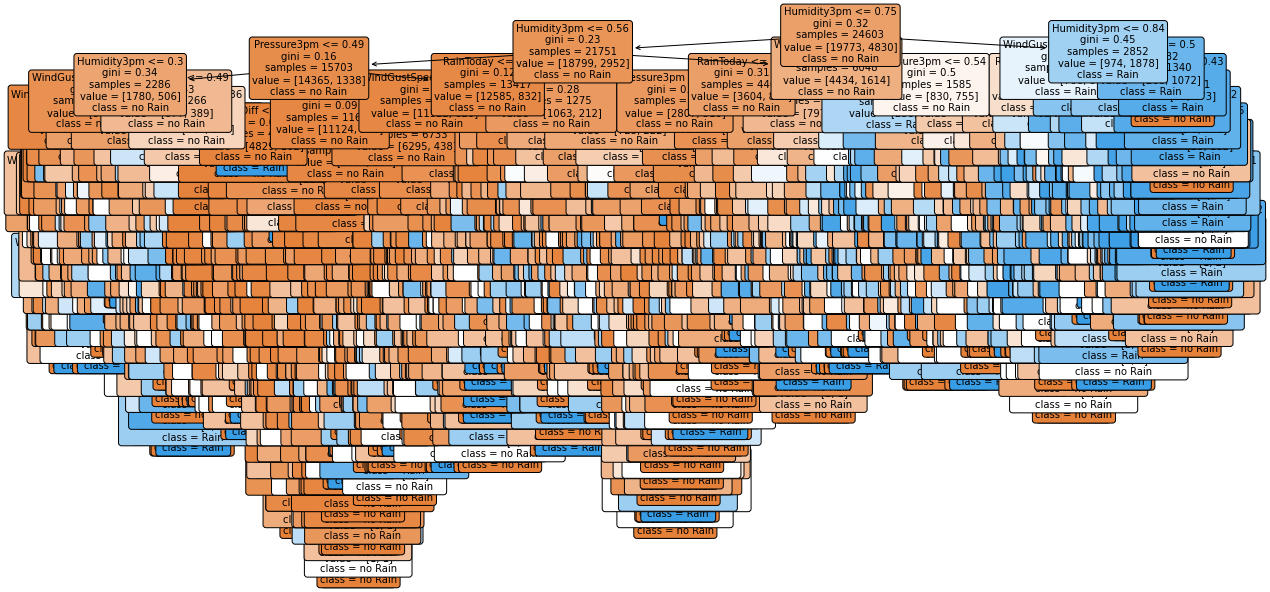
\includegraphics[width = 0.7\textwidth]{Bilder/treedefault}
	\caption{Entschidungsbaum mit Default-Einstellungen}
	\label{fig:treedefault}
\end{figure}
Es ist leicht zu erkennen, dass dieser Baum zu viele Knoten und Blätter enthält. Dem kann mit verschiedenen Einstellungen entgegengewirkt werden.
\subsubsection{Variationen}
Um einen übersichtlichen und brauchbaren Entscheidungsbam erzeugen zu können werden verschiedenen Einstellungen angewandt. Im Folgenden werden ausgewählte Variationen dargestellt und kurz besprochen. Bei der Visualisierung liegt der Fokus auf der Struktur des Baumes und nicht darauf, dass die einzelnen Knoten identifiziert werden können.\\
\begin{figure}[H]
    \centering
     \begin{minipage}{0.30\textwidth}
        \centering
        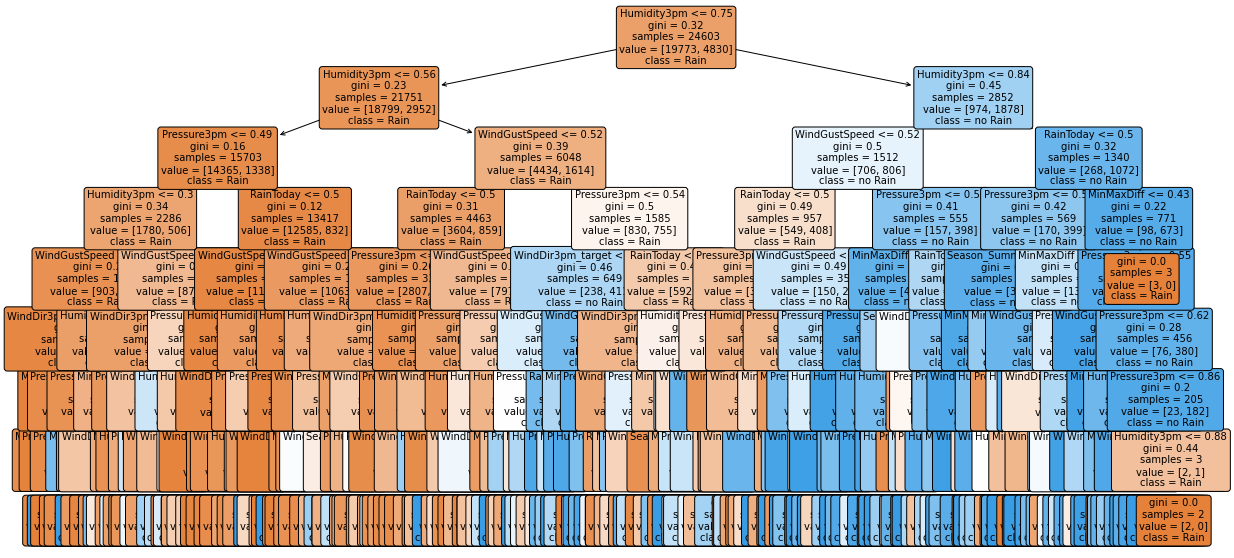
\includegraphics[width=0.9\textwidth]{Bilder/treeMaxDepth8} % first figure itself
        \caption{Maximale Tiefe von 8}
        \label{fig:treeMaxDepth}
    \end{minipage}\hfill
    \begin{minipage}{0.30\textwidth}
        \centering
        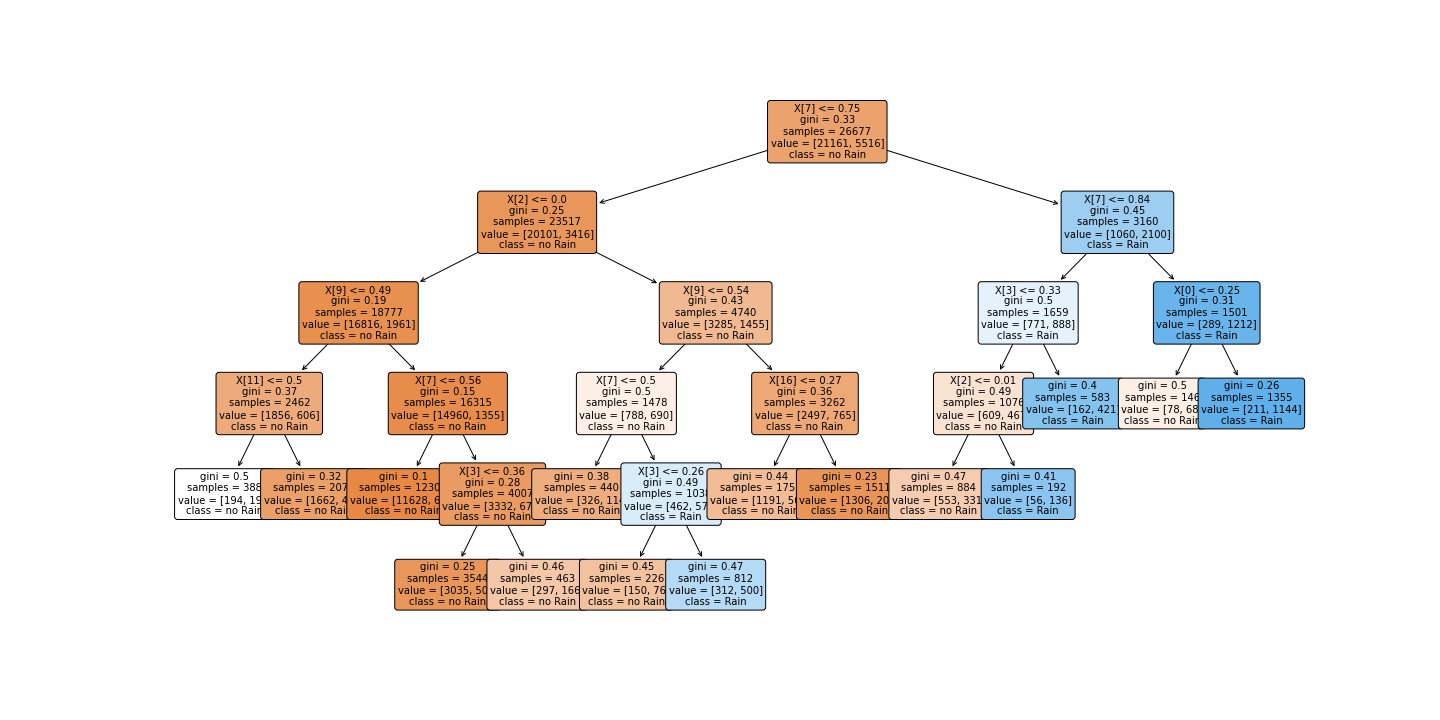
\includegraphics[width=0.9\textwidth]{Bilder/treeMinImpurityDecrease} % first figure itself
        \caption{Minimale Unschärfe Reduktion von 0.003}
        \label{fig:treeMinImpurityDecrease}
    \end{minipage}\hfill
    \begin{minipage}{0.30\textwidth}
        \centering
        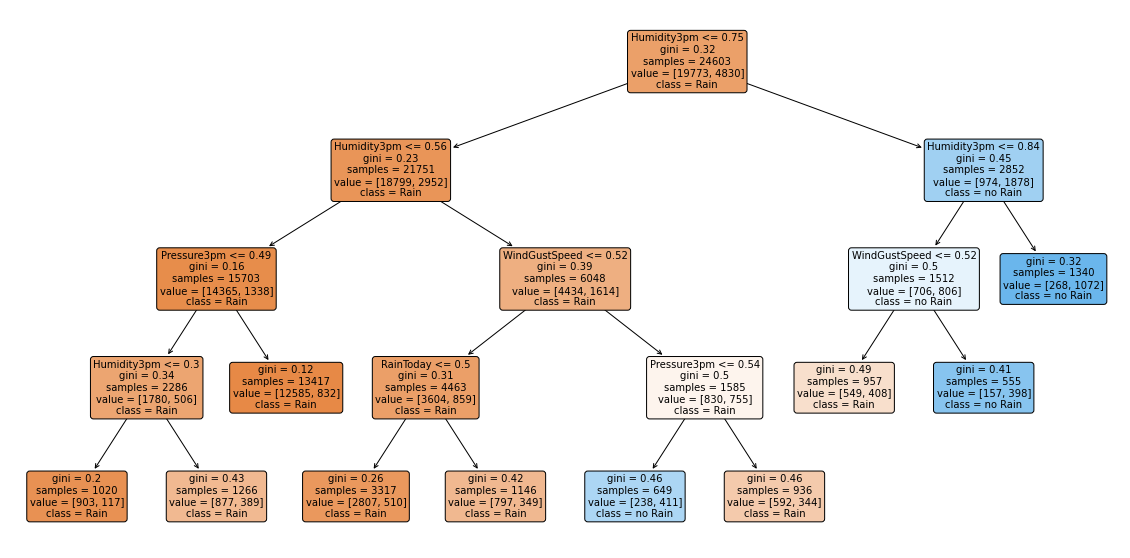
\includegraphics[width=0.9\textwidth]{Bilder/treeMaxLeafNodes} % second figure itself
        \caption{Maximale Blatt-Anzahl von 10}
        \label{fig:treeMaxLeafNodes}
    \end{minipage}
\end{figure}
\noindent \hspace*{7mm}
In Abbildung \ref{fig:treeMaxDepth} wurde eine maximale Tiefe von acht angegeben. Mit dieser Anzahl an Stufen wurde eine bessere Genauigkeit (\emph{accuracy}) und ein geringerer Testfehler erreicht als mit anderen ausprobierten Werten. Trotz der geringen Tiefe ist der Entscheidungsbaum schon sehr unübersichtlich in der Visualisierung. Im Gegensatz zu den anderen Variationen sieht dieser Baum sehr \textbf{symmetrisch}, da jeder Ast gleich lang verfolgt wird und der Baum nicht an unterschiedlichen Tiefen abgeschnitten wird.\\
\noindent \hspace*{7mm}
In den Abbildungen \ref{fig:treeMinImpurityDecrease} und \ref{fig:treeMaxLeafNodes} ist diese Symmetrie nicht mehr zu erkennen. Mit der Einstellung \emph{min\_impurity\_decrease} wird festgelegt, welchen Anteil der Unschärfe ein weiterer Split reduzieren muss. Da das für jeden Knoten einzeln entschieden wird, werden nicht alle Äste bis zur selben Tiefe verfolgt. Bei der Einstellung der maximalen Anzahl an Blatt Knoten ...
\subsubsection{Minimal Cost-Complexity-Pruning}




